\documentclass{beamer} % [aspectratio=169]
\usetheme{ucl}
\setbeamercolor{banner}{bg=darkred}
\setbeamersize{description width=2em}
\setbeamertemplate{navigation symbols}{\vspace{-2ex}} 

%\usepackage{fontspec}
\usepackage[utf8]{inputenc}
% \usepackage[english, greek]{babel}


\usepackage[T1]{fontenc} % Turn £ into $
\usepackage{minted}
\usemintedstyle{emacs}

\usepackage{fancyvrb}
\usepackage{xcolor}
\usepackage{url}

\usepackage{natbib}
\usepackage{bibentry}
\usepackage{url}


\usepackage{tikz}
\usetikzlibrary{positioning}


\newcommand\emc[1]{\textcolor{midred}{\textbf{#1}}}

\AtBeginSection[]{
  \begin{frame}
  \vfill
  \centering
  \begin{beamercolorbox}[sep=8pt,center,shadow=true,rounded=true]{title}
    \usebeamerfont{title}\insertsectionhead\par%
  \end{beamercolorbox}
  \vfill
  \end{frame}
}

\author{Prof.\ Mark Handley, University College London, UK\\
\tiny{Partly based on slides from George Danezis}}
\title{Dynamic Data Structures and Algorithms.}
\subtitle{ENGF0002: Design and Professional Skills }
% \institute{}
\date{Term 1, 2018}


\begin{document}
\nobibliography*


\frame{
\titlepage
}

\begin{frame}
\frametitle{Sorting.}

Binary search, and a number of other efficient algorithms, rely on sorted sequences. 

\vspace{3mm}
We next study:
\begin{itemize}
	\item A simple sorting algorithm. %, \emc{bubble sort}.
	\item A better sorting algorithm, \emc{merge sort}.
	\item The \emc{time complexity} of sorting.
	\item How to show sorting is \emc{correct}.
	% \item Issues around maintaining \emc{large sorted indexes}.
	\item How to write \emc{generic} sorting and searching algorithms.
\end{itemize}

\end{frame}

\begin{frame}
  %\frametitle{Bubble Sort}
  \centering
  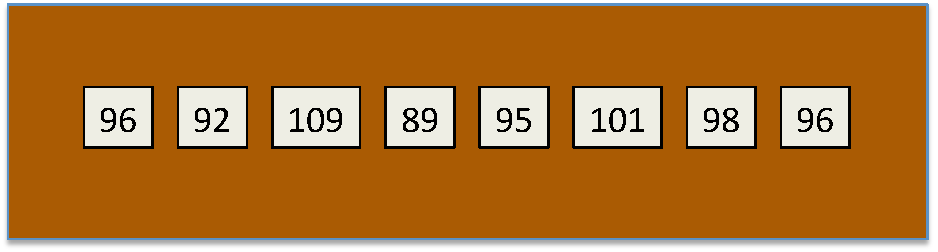
\includegraphics[width=70mm]{assets/swapping1-cropped.pdf}
\end{frame}
\begin{frame}
  %\frametitle{Bubble Sort}
  \centering
  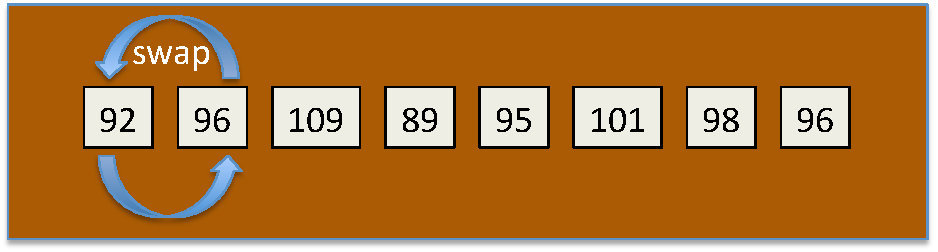
\includegraphics[width=70mm]{assets/swapping2-cropped.pdf}
\end{frame}
\begin{frame}
  %\frametitle{Bubble Sort}
  \centering
  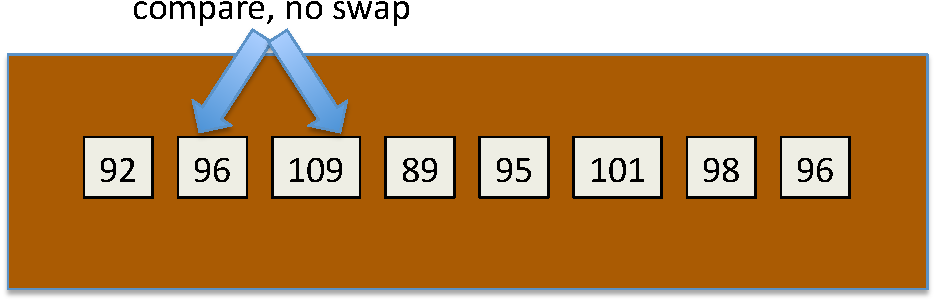
\includegraphics[width=70mm]{assets/swapping3-cropped.pdf}
\end{frame}
\begin{frame}
  \frametitle{Bubble Sort}
  \centering
  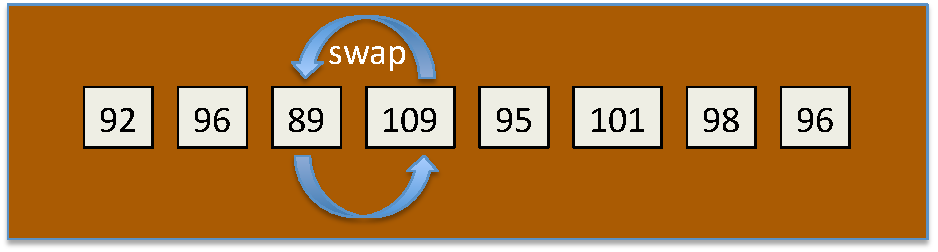
\includegraphics[width=70mm]{assets/swapping4-cropped.pdf}
\end{frame}
\begin{frame}
  \frametitle{Bubble Sort}
  \centering
  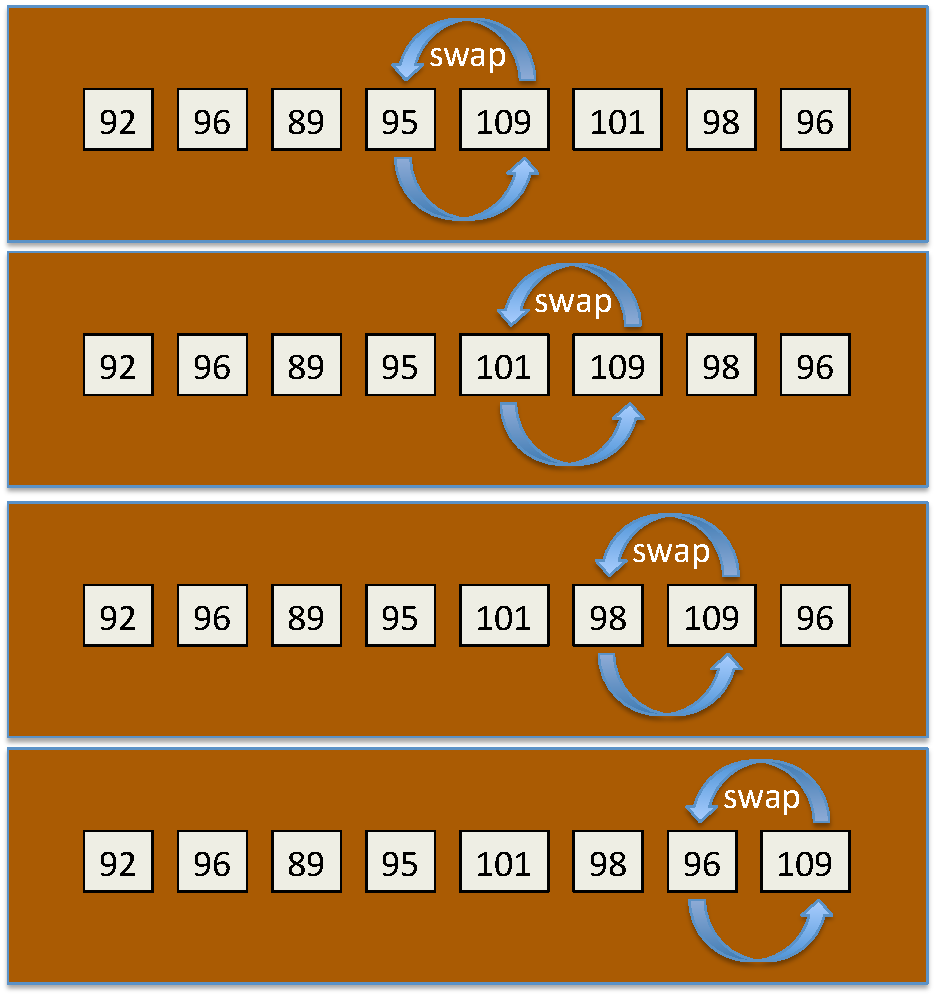
\includegraphics[width=70mm]{assets/swapping5-cropped.pdf}
\end{frame}
\begin{frame}
  \frametitle{Bubble Sort}
  \centering
  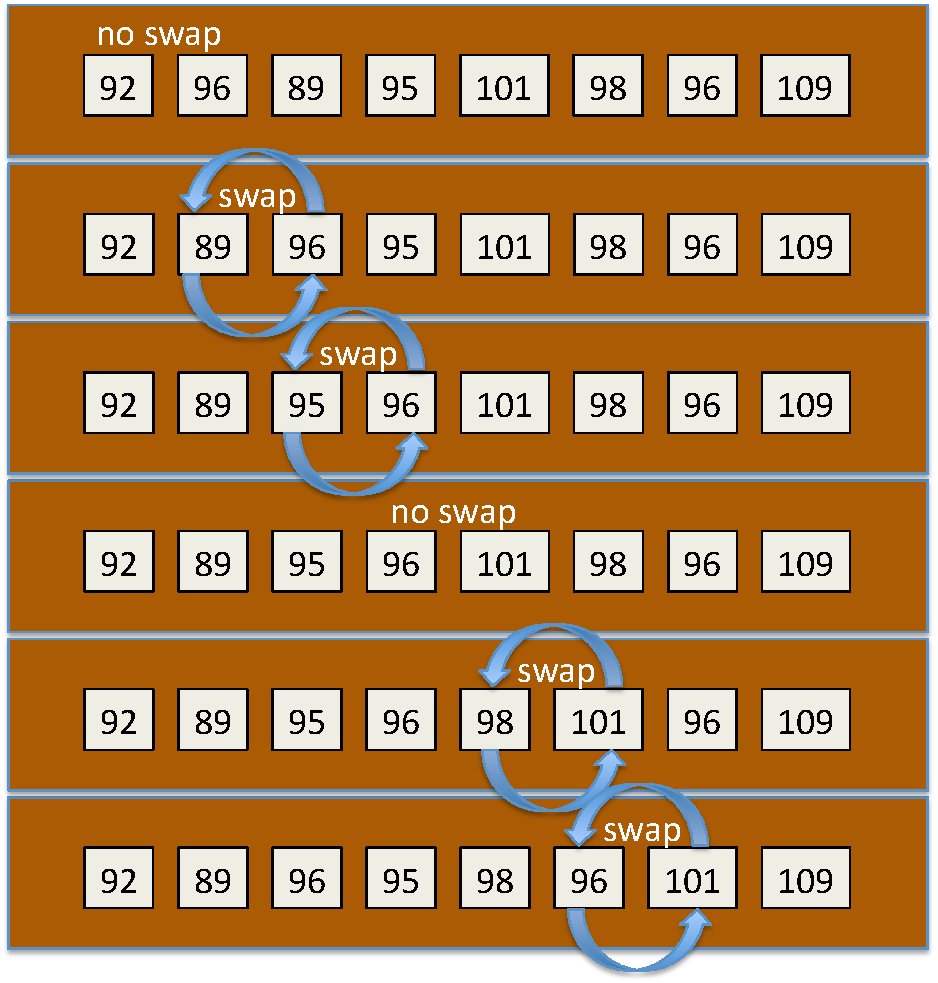
\includegraphics[width=70mm]{assets/swapping6-cropped.pdf}
\end{frame}
\begin{frame}
  \frametitle{Bubble Sort}
  \centering
  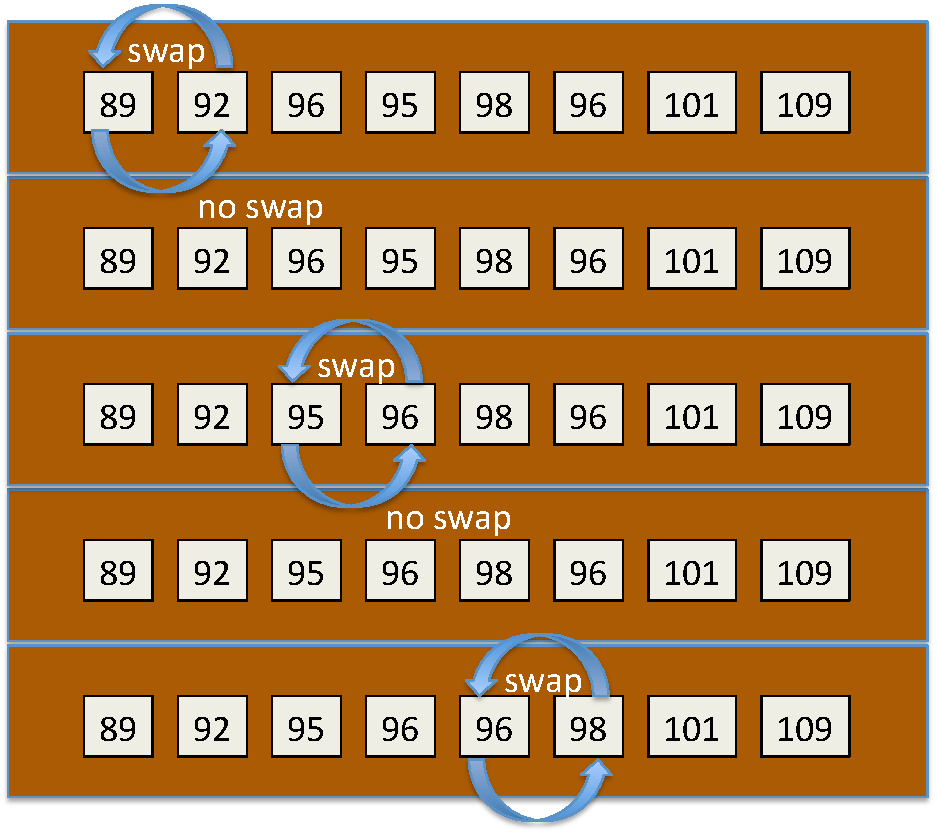
\includegraphics[width=70mm]{assets/swapping7-cropped.pdf}
\end{frame}
\begin{frame}
  \frametitle{Visualizing Bubble Sort}
  \centering
  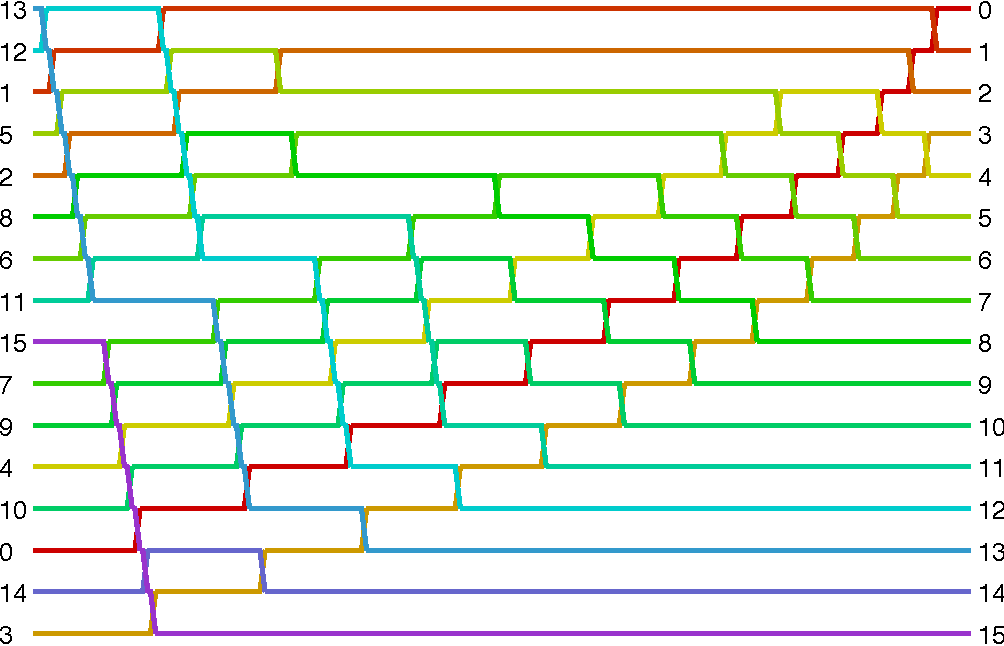
\includegraphics[width=100mm]{assets/bubblesort.pdf}
\end{frame}
\begin{frame}
  \frametitle{Visualizing Bubble Sort}
  \centering
  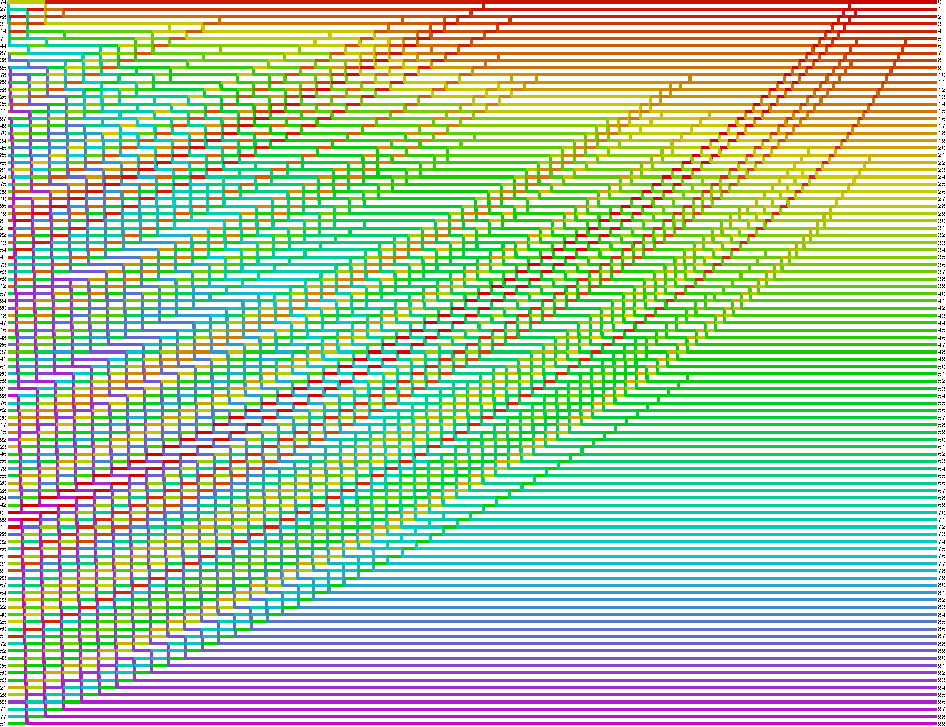
\includegraphics[width=100mm]{assets/bubblesort2.pdf}
\end{frame}

\begin{frame}
  \frametitle{Complexity of Bubble Sort}
  What is the computational complexity of Bubblesort with $n$ items?
  \begin{itemize}
  \item Each pass through the data involves $n-1$ comparisons.
  \item Each pass moves one more item to the end of the list.
    \begin{itemize}
    \item After 1 pass, the largest item is at the end.
    \item After 2 passes, the largest two items are at the end and sorted.
    \item After $k$ passes, the largest $k$ items are at the end and sorted.
    \end{itemize}
  \item After $n$ passes, the whole list is sorted.
  \end{itemize}
  \vspace{3mm}
  Requires $n(n-1)$ comparisons.

  \vspace{3mm}
  $n(n-1) = n^2 - n = \mathcal{O}(n^2)$
\end{frame}

\begin{frame}
  \frametitle{Optimization of Bubblesort}
  Observe we don't need to compare all $n$ items in each pass.
  \begin{itemize}
  \item In pass $k$, the last $k-1$ items are already sorted, so we can stop the pass early.
  \item Cuts the total number of comparisons in half.
  \end{itemize}
  Does this change the complexity?
\end{frame}

\begin{frame}
  \frametitle{Merging lists}
  \centering
  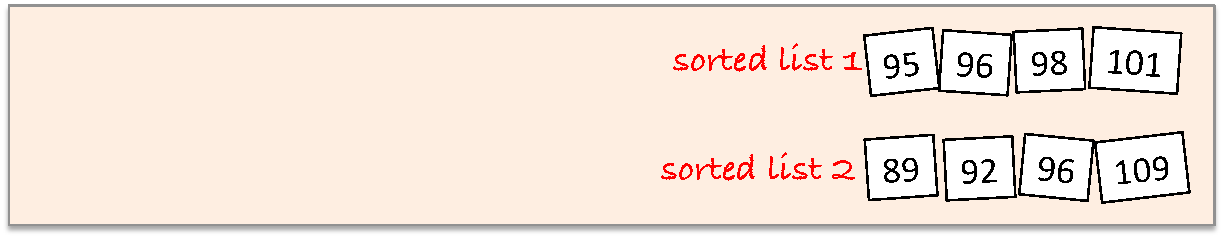
\includegraphics[width=100mm]{assets/merge-move0-crop.pdf}
\end{frame}

\begin{frame}
  \frametitle{Merging lists}
  \centering
  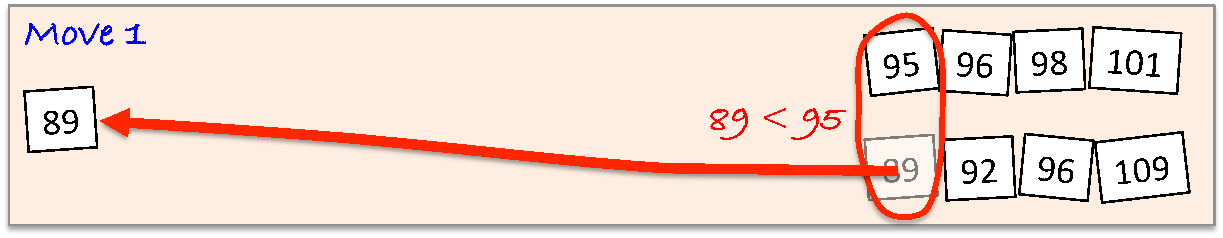
\includegraphics[width=100mm]{assets/merge-move1-crop.pdf}
\end{frame}

\begin{frame}
  \frametitle{Merging lists}
  \centering
  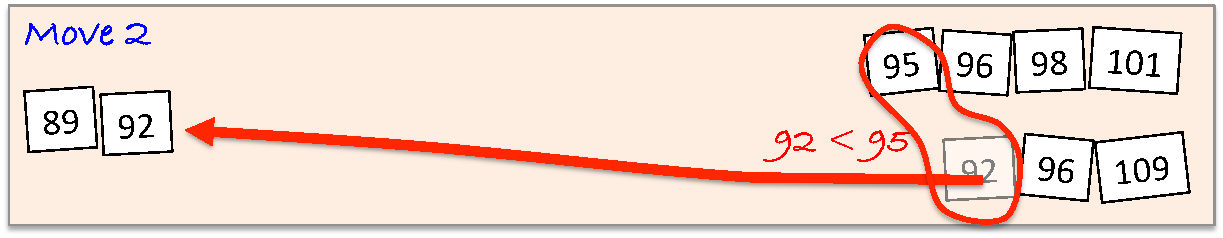
\includegraphics[width=100mm]{assets/merge-move2-crop.pdf}
\end{frame}

\begin{frame}
  \frametitle{Merging lists}
  \centering
  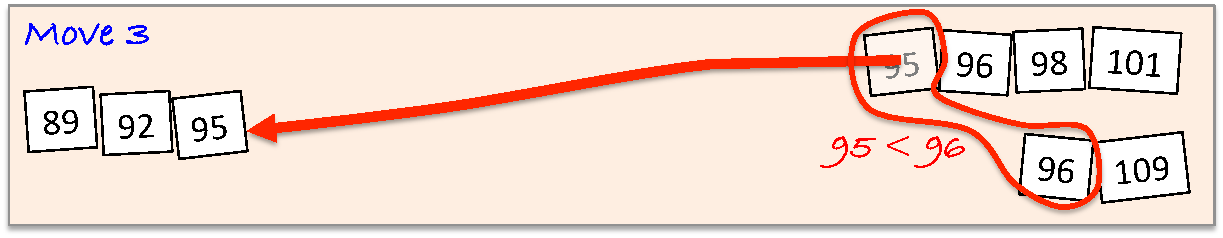
\includegraphics[width=100mm]{assets/merge-move3-crop.pdf}
\end{frame}

\begin{frame}
  \frametitle{Merging lists}
  \centering
  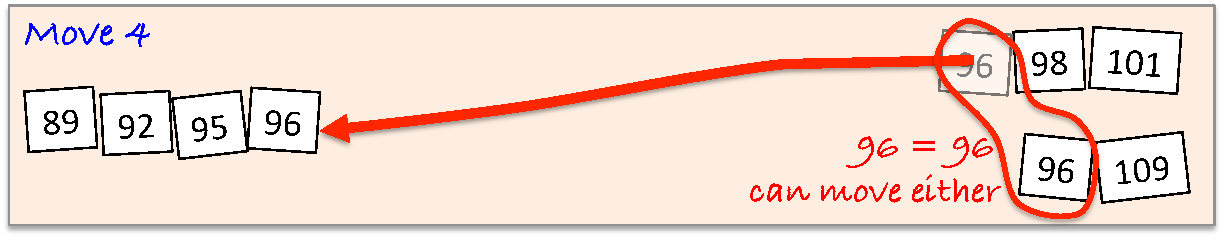
\includegraphics[width=100mm]{assets/merge-move4-crop.pdf}
\end{frame}

\begin{frame}
  \frametitle{Merging lists}
  \centering
  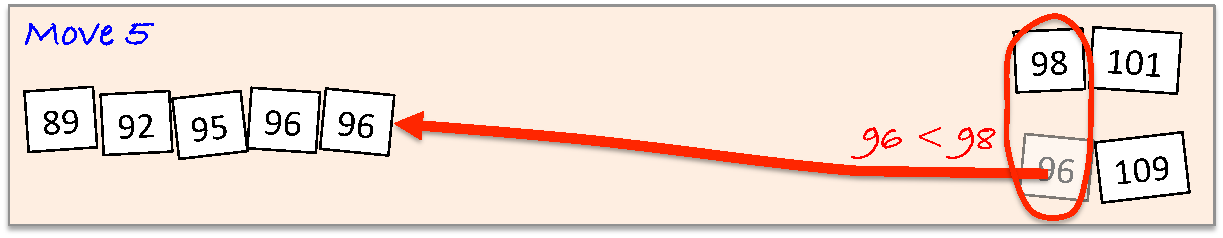
\includegraphics[width=100mm]{assets/merge-move5-crop.pdf}
\end{frame}

\begin{frame}
  \frametitle{Merging lists}
  \centering
  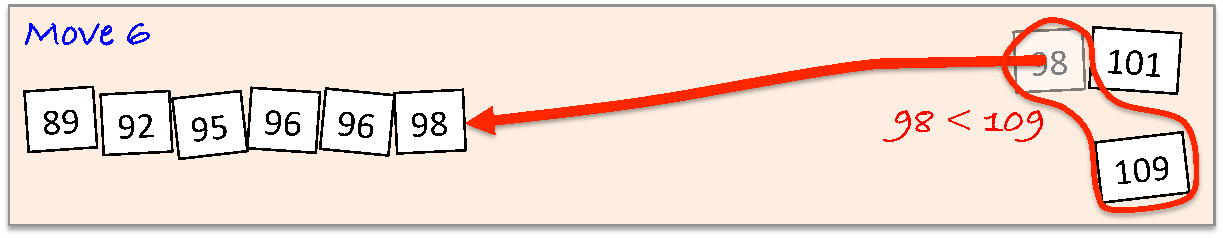
\includegraphics[width=100mm]{assets/merge-move6-crop.pdf}
\end{frame}

\begin{frame}
  \frametitle{Merging lists}
  \centering
  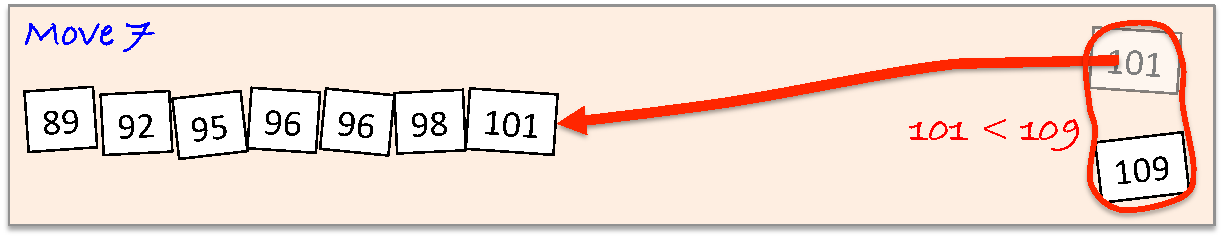
\includegraphics[width=100mm]{assets/merge-move7-crop.pdf}
\end{frame}

\begin{frame}
  \frametitle{Merging lists}
  \centering
  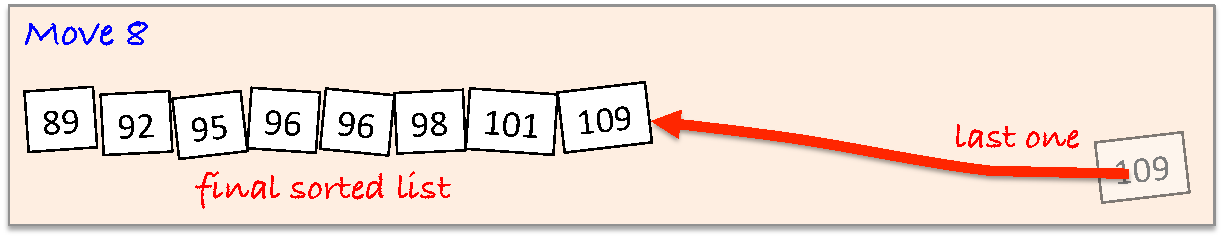
\includegraphics[width=100mm]{assets/merge-move8-crop.pdf}

  \begin{block}{Observation}
    Merging two \emc{already sorted} lists containing $n$ items only requires $n-1$ comparisons and $n$ moves.
    \end{block}
\end{frame}

\begin{frame}
  \frametitle{Little lists}
  \centering
  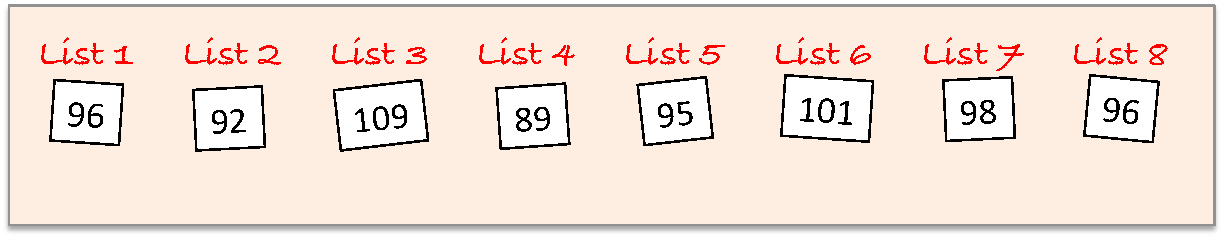
\includegraphics[width=100mm]{assets/merge-move9-crop.pdf}
  \begin{block}{Observation}
    Lists of length 1 are \emc{already sorted!}.
    \end{block}
\end{frame}

\begin{frame}
  \frametitle{Merging lists (round 1)}
  \centering
  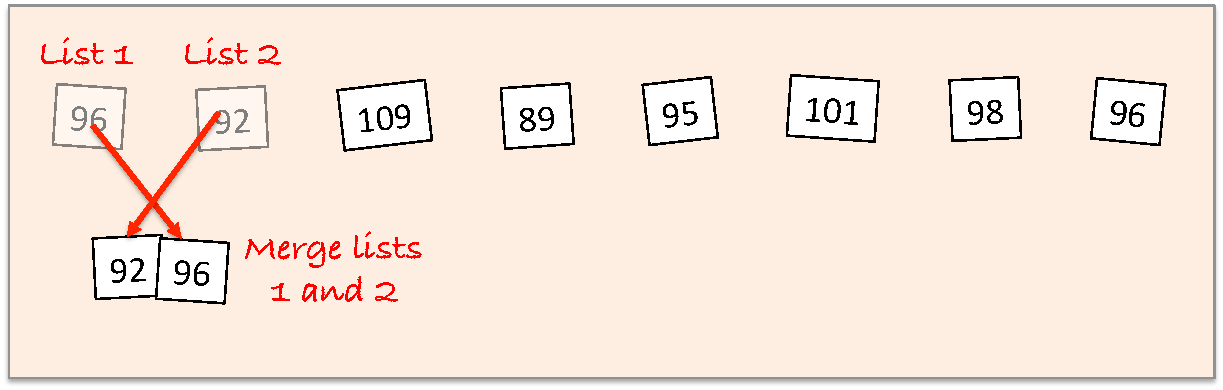
\includegraphics[width=100mm]{assets/merge-move10-crop.pdf}
\end{frame}

\begin{frame}
  \frametitle{Merging lists (round 1 continued)}
  \centering
  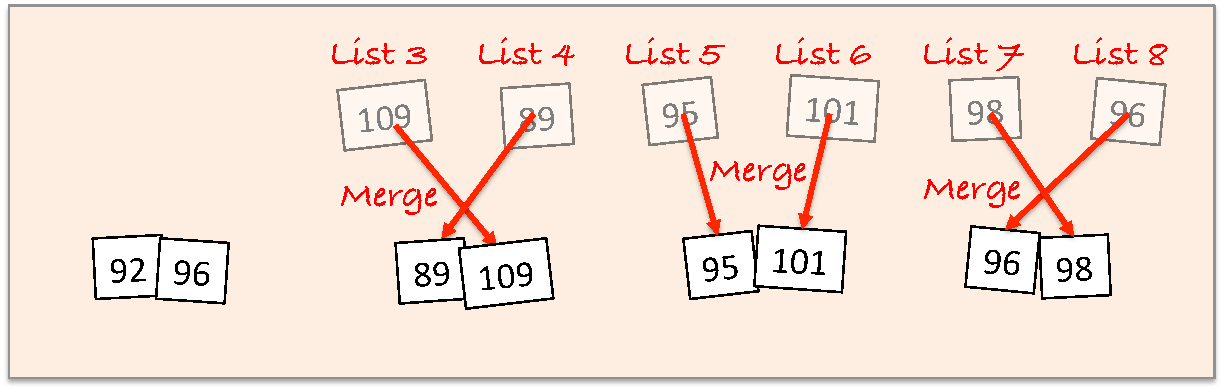
\includegraphics[width=100mm]{assets/merge-move11-crop.pdf}
\end{frame}

\begin{frame}
  \frametitle{Merging lists (round 2)}
  \centering
  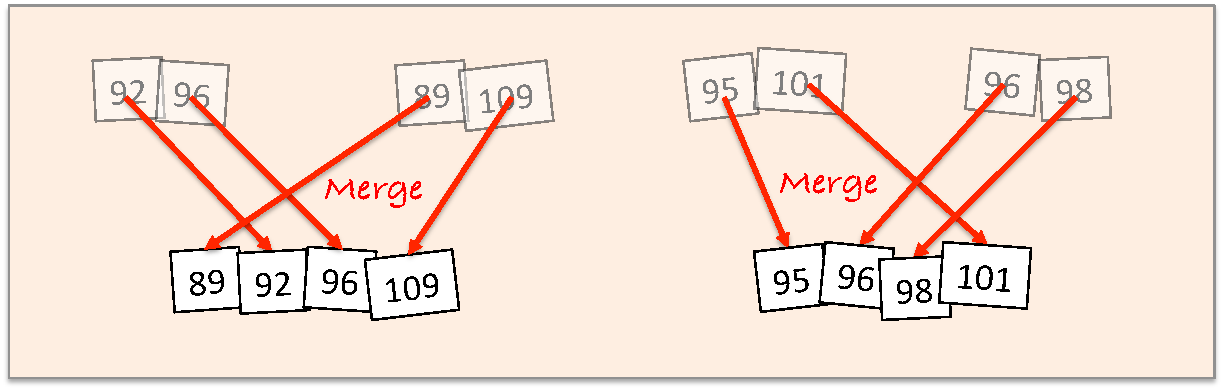
\includegraphics[width=100mm]{assets/merge-move12-crop.pdf}
\end{frame}

\begin{frame}
  \frametitle{Merging lists (round 3)}
  \centering
  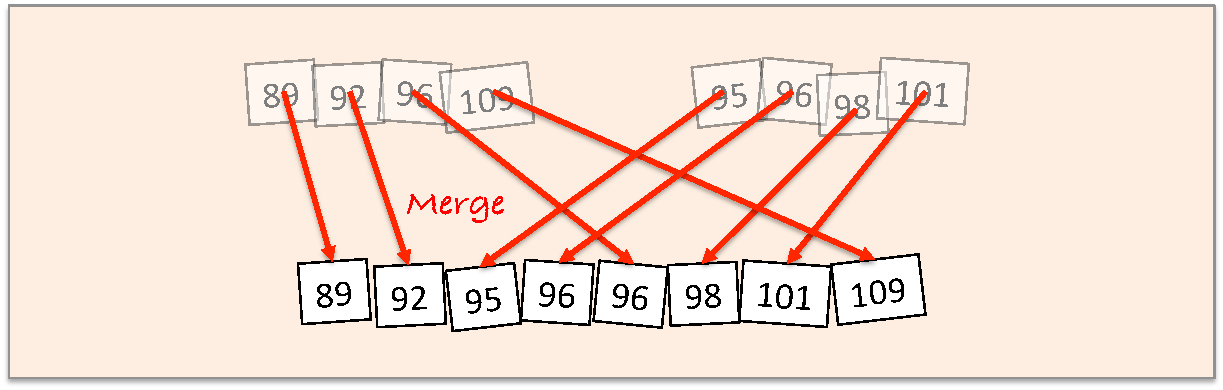
\includegraphics[width=100mm]{assets/merge-move13-crop.pdf}
\end{frame}

\begin{frame}
  \frametitle{Visualizing merging lists: 64 items}
  \centering
  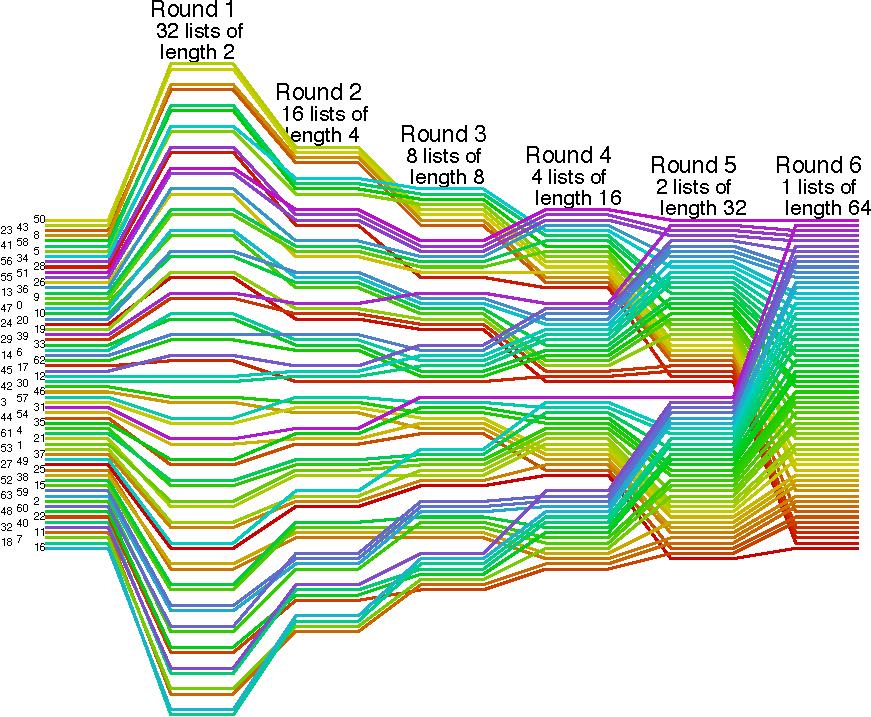
\includegraphics[width=90mm]{assets/mergesort.pdf}
\end{frame}

\begin{frame}
  \frametitle{Visualizing merging lists: 64 items}
  \centering
  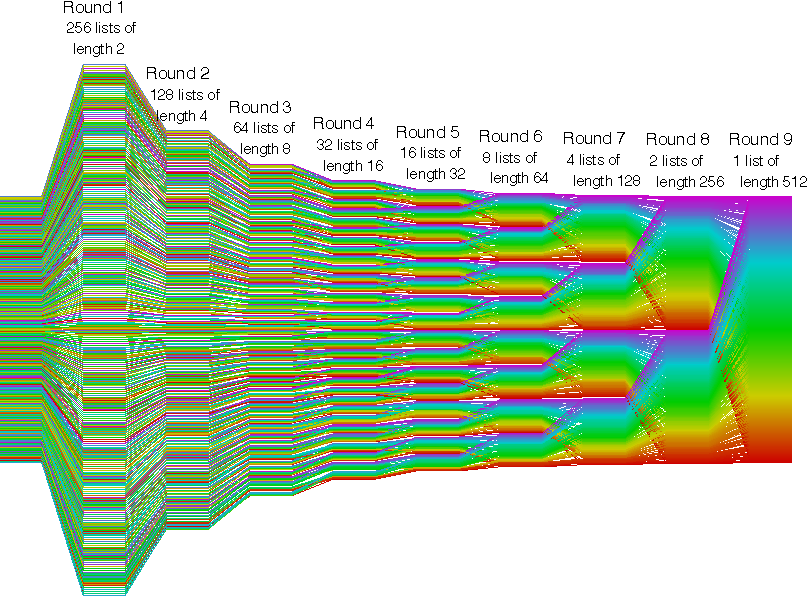
\includegraphics[width=90mm]{assets/mergesort2.pdf}
\end{frame}

\begin{frame}
\frametitle{Merge sort}

Mergesort was proposed by John von Neumann in 1945.

\vspace{3mm}
Essentially two algorithms:

\vspace{5mm}
Algorithm 1. Merge two sorted lists into one sorted list:
\begin{itemize}
\item While both lists are not empty, consider the first unprocessed item from both.
\item Add to the front of the new list the smaller or available one, and remove it from its list. Repeat.
\item Append remaining elements of one of the lists.
\end{itemize}

\end{frame}

\begin{frame}
\frametitle{Merge sort}

Algorithm 2. Merge Sort.
\begin{itemize}
\item If the list has length 1, we're done.
\item Otherwise, divide into two sub-lists of equal length.
\item Merge Sort both lists separately.
\item Merge the two sorted lists using Algorithm 1.
\end{itemize}

\end{frame}

\begin{frame}
\frametitle{Tests for sorting.}

	\inputminted[
		% firstline=10,
		lastline=14,
		xleftmargin=1.4em,
		%frame=lines,
		%framesep=2mm,
		%baselinestretch=1.2,
		bgcolor=stone,
		fontsize=\footnotesize,
		%linenos
	]{python}{src/mergesort.py}

\end{frame}

\begin{frame}
\frametitle{Merge two sorted lists (algorithm 1).}

	\inputminted[
		firstline=25,
		lastline=42,
		xleftmargin=0.0em,
		%frame=lines,
		%framesep=2mm,
		%baselinestretch=1.2,
		bgcolor=stone,
		fontsize=\footnotesize,
		%linenos
	]{python}{src/mergesort.py}

\end{frame}

\begin{frame}
\frametitle{A recursive implementation of mergesort  (algorithm 2).}

	\inputminted[
		firstline=17,
		lastline=23,
		xleftmargin=1.4em,
		%frame=lines,
		%framesep=2mm,
		%baselinestretch=1.2,
		bgcolor=stone,
		fontsize=\footnotesize,
		%linenos
	]{python}{src/mergesort.py}

\begin{itemize}
\item Python \emc{slicing}: \texttt{lst[start:end]} returns the list from index \texttt{start} up to, but not including, index \texttt{end}. If omitted from zero to the length of the list.
\item Use \texttt{lst.copy()} to get a new \emc{copy} of the list (otherwise we'll just modify the original!).
\end{itemize}

\end{frame}

\begin{frame}
\frametitle{How to argue mergesort is correct.}

Structural induction (verbal reasoning): 
\begin{itemize}
	\item Argue that the merge operation is correct: given two sorted lists it produces a sorted list.
	\item Base case of mergesort: a single element list is sorted.
	\item Inductive case of mergesort: assume mergesort for a previous step works, prove that the result is sorted. Follows from the properties of merge.
\end{itemize}

\vspace{3mm}
Note that the recursive structure of the program supports the argument of correctness through induction.

\end{frame}

\begin{frame}
\frametitle{What is the cost of mergesort.}

The time complexity of merge (algorithm 1) is $\mathcal{O}(n)$, where $n$ is the sum of the lengths of both lists.

\vspace{3mm}

Mergesort (algorithm 2) can only divide an array of $n$ elements $\mathcal{O}(\log n)$ times. At each level of subdivision the overall costs of the merge operations will be $\mathcal{O}(n)$ (total from algorithm 1).

\vspace{3mm}
Therefore the overall time complexity of mergesort is of the \emc{order $\mathcal{O}(n \log n)$}. 

\vspace{3mm}
This is \emc{optimal} for comparison based algorithms (but note that \emc{constant factors may vary}.) Space complexity may also vary.

\end{frame}

\section{More sequences and generic programming}

\begin{frame}
\frametitle{Strings and byte sequences.}

Besides \emc{lists}, Python supports a number of other sequence types:
\begin{itemize}
        \item \emc{tuples}: like a list, but content is immutable once assigned.
	\item \emc{strings} (\texttt{str}): represent sequences of unicode characters.
	\item \emc{bytes} (\texttt{bytes}): represent a sequences of raw bytes (ie. values from 0 to 255).
	\item Strings are transformed into and from sequences of bytes through an \emc{encoding} such as \texttt{utf8} or \texttt{ASCII}.
\end{itemize}

	\inputminted[
		firstline=3,
		lastline=5,
		xleftmargin=1.4em,
		%frame=lines,
		%framesep=2mm,
		%baselinestretch=1.2,
		bgcolor=stone,
		fontsize=\footnotesize,
                style=bw,
		%linenos
	]{python}{src/strbytes.py} 

\end{frame}

\begin{frame}
\frametitle{Internationalization (i18n).}

Old encodings such as ASCII only map latin characters to bytes. Others cannot exist!

\vspace{3mm}
Software and services need to be \emc{accessible to all people in their native languages}. Always use string representations that can represent all languages (and emoji!) such as \emc{unicode}, and encodings into bytes such as \emc{utf-8} to represent those strings as bytes.

\begin{itemize}
\item Don't assume English is the only possible language.
\item Plan for internationalization: do not hard code english strings into software, but rather load them from a file that can be localized.
\item Dates, currency, number representations also vary per locale.
\end{itemize}

\end{frame}

\begin{frame}
\frametitle{Operations on string.}

Strings support a number of operations:
	\inputminted[
		firstline=7,
		lastline=17,
		xleftmargin=-1.4em,
		%frame=lines,
		%framesep=2mm,
		%baselinestretch=1.2,
		bgcolor=stone,
		fontsize=\footnotesize,
                style=bw,
		%linenos
	]{python}{src/strbytes.py} 

For full reference see: \url{https://docs.python.org/3.7/library/string.html}

\end{frame}

\begin{frame}
\frametitle{String literals \& formatting.}

\begin{itemize}
\item String constants in programs can be encosed in single or double quotes.
\item You can represent special characters in strings using the \texttt{`\textbackslash'} symbol, such as new line as \texttt{{\textbackslash}n} and tab as \texttt{{\textbackslash}t}.
\item The \texttt{format} method substitutes into the string:
\end{itemize}

	\inputminted[
		firstline=19,
		lastline=25,
		xleftmargin=-1.4em,
		%frame=lines,
		%framesep=2mm,
		%baselinestretch=1.2,
		bgcolor=stone,
		fontsize=\footnotesize,
                style=bw,
		%linenos
	]{python}{src/strbytes.py} 


\end{frame}

\begin{frame}
\frametitle{Generic programming: how to sort a list of strings.}

Do you need to \emc{re-implement mergesort} for lists of strings? Remember the \emc{abstraction principle}.

\vspace{5mm}
However our implementation of mergesort seems to just work:
	\inputminted[
		firstline=29,
		lastline=33,
		xleftmargin=1.4em,
		%frame=lines,
		%framesep=2mm,
		%baselinestretch=1.2,
		bgcolor=stone,
		fontsize=\footnotesize,
		%linenos
	]{python}{src/strbytes.py}

\emc{Generic programming} ensures that algorithms are independent of and agnostic about the exact types they are processing.


\end{frame}

\begin{frame}
\frametitle{Why generic programming works.}

Merge (algorithm 1) only uses `\texttt{<=}' on items within the list to sort:
	\inputminted[
		firstline=32,
		lastline=41,
		xleftmargin=0em,
		%frame=lines,
		%framesep=2mm,
                highlightcolor=yellow,
		highlightlines={36},
		%baselinestretch=1.2,
		bgcolor=stone,
		fontsize=\footnotesize,
		%linenos
	]{python}{src/mergesort.py}

If the operation less-than-or-equal (compare) is supported correctly by the type of object in the list, mergesort will return the correct result.

\end{frame}

\begin{frame}
\frametitle{Sorting strings by length, rather than lexicographically.}

Strategy: allow the programmer to specify a function that performs a comparison. Parametrize mergesort by the comparison function.

	\inputminted[
		firstline=20,
		lastline=26,
		xleftmargin=1.4em,
		%frame=lines,
		%framesep=2mm,
                highlightcolor=yellow,
		highlightlines={20,24-26},
		%baselinestretch=1.2,
		bgcolor=stone,
		fontsize=\footnotesize,
		%linenos
	]{python}{src/mergesort_cmp.py}



\end{frame}

\begin{frame}
% \frametitle{Sorting strings by length, rather than lexicographically.}

	\inputminted[
		firstline=28,
		lastline=44,
		xleftmargin=0.4em,
		%frame=lines,
		%framesep=2mm,
                highlightcolor=yellow,
		highlightlines={34},
		%baselinestretch=1.2,
		bgcolor=stone,
		fontsize=\footnotesize,
		%linenos
	]{python}{src/mergesort_cmp.py}


\end{frame}

\begin{frame}
\frametitle{Example of different comparison functions for strings.}

	\inputminted[
		firstline=46,
		lastline=57,
		xleftmargin=1.4em,
		%frame=lines,
		%framesep=2mm,
                bgcolor=stone,
		fontsize=\footnotesize,
		%linenos
	]{python}{src/mergesort_cmp.py}

\end{frame}

\begin{frame}
\frametitle{Functions are just variables.}

\begin{block}{Functions are first-class objects.}
In modern programming languages functions are first-class objects (of type \texttt{function}). They are assigned to names, and they can be passed as arguments to function calls; stored in data structures; etc. 
\end{block}

The shorthand \texttt{lambda} notation can be used to define functions within expressions.
	\inputminted[
		firstline=59,
		lastline=64,
		xleftmargin=1.4em,
		%frame=lines,
		%framesep=2mm,
		fontsize=\footnotesize,
                bgcolor=stone,
		%linenos
	]{python}{src/mergesort_cmp.py}


\end{frame}

\section{Visualization Diversion}

\begin{frame}
  %\frametitle{Flow Charts}
  \centering
  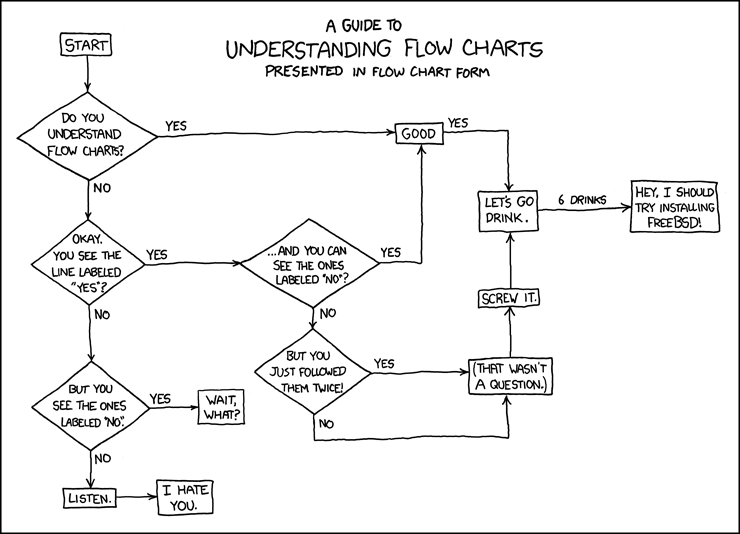
\includegraphics[width=110mm]{assets/flow_charts}
\end{frame}

\begin{frame}
  \frametitle{Cumulative Distribution Functions (CDFs)}
  \centering
  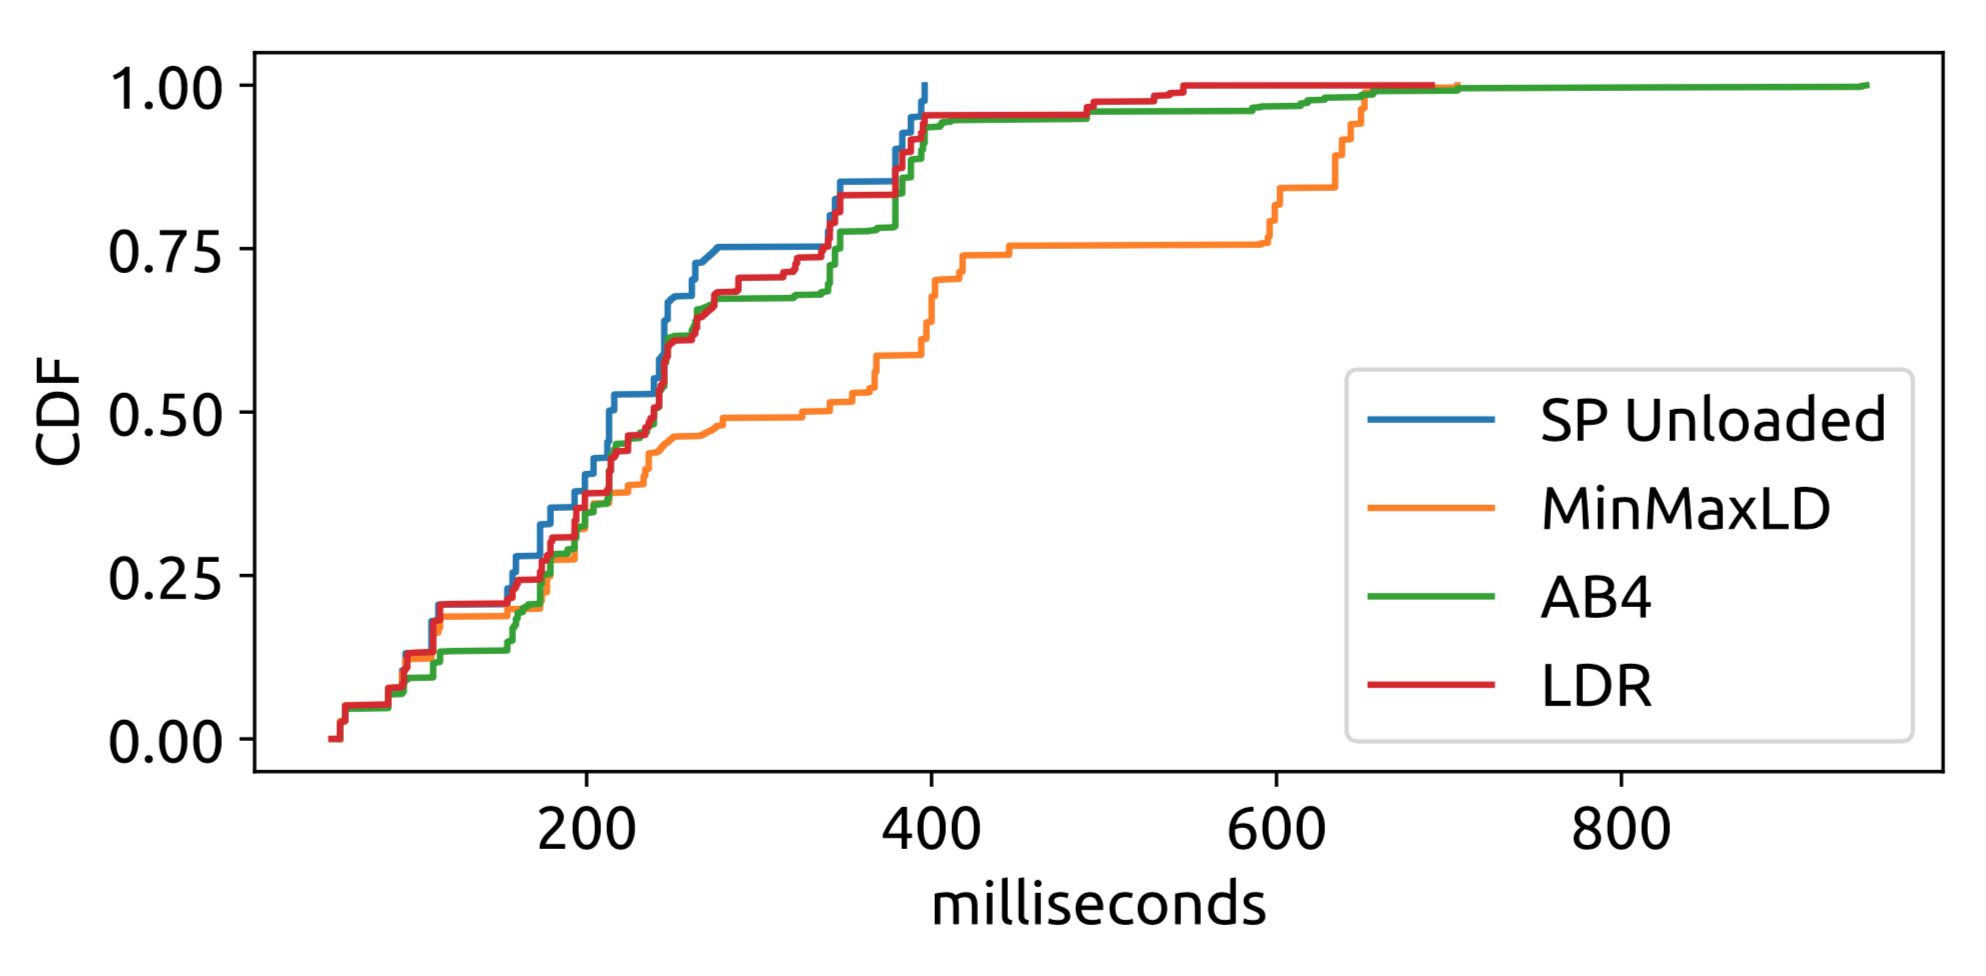
\includegraphics[width=110mm]{assets/cdf}

  y value shows the cumulative fraction of data values less than the x value
\end{frame}

\bibliographystyle{alpha}
\nobibliography{references}

\end{document}
